\Chapter{Koncepció}


	\Section{Lineáris egyenletrendszerek}
	
	
	A lineáris programozási feladatokban mind a célfüggvény, mind a feltételeket meghatározó függvények az $x_1, x_2,\ldots ,x_n$ döntési változók lineáris függvényei. A kényszerfeltételek megadhatók lineáris egyenlőség vagy egyenlőtlenség formájában, és az egyes döntési változók előjelére is lehetnek megkötések. Így azonban még mindig rengeteg változata lehet az LP-problémáknak, amelyekre mindannyiunknak különböző megoldási módszereket kell konstruálnunk. A következőkben megmutatjuk, hogy a probléma optimális megoldásának létezése és meghatározása szempontjából elegendő egy speciális LP-probléma, az ún. standard probléma vizsgálatára szorítkozni. Egy lineáris programozási feladatot akkor nevezünk standard feladatnak, ha a következő formában van megadva: 
	
$$c^Tx \rightarrow \max$$
$$Ax=b, (b\geq0)$$
$$x \geq0$$	
ahol

$c=(c_1,c_2,\ldots,c_n)^T$ a vektor a célfügvény együtthatóiból áll

%%Melohelyen


Lépések sorozata egy általános LP-feladat szabványos formává alakításához:

Minimális probléma esetén a problémát maximális problémává alakítjuk át úgy, hogy a célfüggvény együtthatóit megszorozzuk (-1)-gyel, mivel az f (x) célfüggvénynek abban az x pontban van minimuma, ahol a -f (x) célfüggvény maximális. 

Ha a k-adik feltétel jobb oldalán lévő bk konstans negatív, akkor a teljes feltételes egyenlőség vagy egyenlőtlenség (-1)-szeresét vesszük. 

Ha az xi döntési változónak nincs nemnegatív feltétele, akkor ezt a változót két újonnan bevezetett nemnegatív változó különbségeként írjuk fel: xi = x ′ -x ′ ′.
Ha az xj ≤ 0 feltétel van megadva, akkor a változó ellenkezőjét a nem negatív ̃xj = -xj változó bevezetésével számítjuk ki. 

Ha a k-adik kényszer ≤ egyenlőtlenség az ak1x1 + ak2x2 + ... formában adott. + aknxn ≤bk, akkor egy nemnegatív uk segédváltozó hozzáadásával adunk hozzá egy egyenletet: 

ak1x1 + ak2x2 + ... + aknxn + uk = bk

Ha az l-edik kényszer ≥ egyenlőtlenség az al1x1 + al2x2 + ... formában. + alnxn ≥ bl, akkor egyenlőséggé alakítjuk át egy nem negatív v1 segédváltozó kivonásával. 

al1x1 + al2x2 + ... + alnxn −vl = b

	
	
	\Section{Hátizsák probléma}
	A knapsack-probléma a kombinatorikus optimalizálás egyik problémája: A feladat a következő: Adott egy halmaznyi elem, amelyek mindegyikének van egy súlya és egy értéke, határozza meg, hogy hány darabot kell felvenni a gyűjteménybe úgy, hogy az összes súly kisebb vagy egyenlő legyen egy adott határértéknél, és az összes érték a lehető legnagyobb legyen. Nevét arról a problémáról kapta, amellyel az szembesül, akinek egy meghatározott méretű hátizsákot kell megtömnie a legértékesebb tárgyakkal. A probléma gyakran felmerül az erőforrás-elosztás során, amikor a döntéshozóknak nem osztható projektek vagy feladatok halmazából kell választaniuk egy rögzített költségvetés, illetve időkorlátozás mellett.
	
	A hátizsákproblémát több mint egy évszázada tanulmányozzák, a korai munkák már 1897-ben megjelentek.[1] A "hátizsákprobléma" elnevezés Tobias Dantzig (1884-1956) matematikus korai munkáira vezethető vissza,[2] és arra a hétköznapi problémára utal, hogy a legértékesebb vagy leghasznosabb tárgyakat úgy kell becsomagolni, hogy a poggyász ne legyen túlterhelve. 
	
	\SubSection{Alkalmazása}
	
	A Knapsack-problémák számos területen megjelennek a valós döntéshozatali folyamatokban, például a nyersanyagok legkevésbé pazarló darabolásának megtalálása, befektetések és portfóliók kiválasztása, eszközök kiválasztása eszközfedezetű értékpapírosításhoz, valamint kulcsok generálása a Merkle-Hellman és más Knapsack-krip\-to\-szisz\-té\-mák\-hoz.
	
	A knapsack-algoritmusok egyik korai alkalmazása olyan tesztek szerkesztésében és pontozásában volt, amelyekben a tesztelők választhatnak, hogy milyen kérdésekre válaszolnak. Kis példák esetén meglehetősen egyszerű folyamat a tesztelőknek ilyen választási lehetőséget biztosítani. Ha például egy vizsga 12 kérdést tartalmaz, amelyek mindegyike 10 pontot ér, a vizsgázónak csak 10 kérdésre kell válaszolnia ahhoz, hogy elérje a maximálisan elérhető 100 pontot. A pontértékek heterogén eloszlásával rendelkező tesztek esetében azonban nehezebb választási lehetőséget biztosítani. Feuerman és Weiss egy olyan rendszert javasolt, amelyben a tanulók heterogén tesztet kapnak összesen 125 lehetséges pontszámmal. A tanulóknak az összes kérdésre a legjobb tudásuk szerint kell válaszolniuk. A feladatok lehetséges részhalmazai közül, amelyek összpontszáma 100 pontot tesz ki, egy knapsack-algoritmus meghatározná, hogy melyik részhalmaz adja az egyes tanulóknak a lehető legmagasabb pontszámot.
	
	A Stony Brook University Algorithm Repository (Stony Brook Egyetem Algoritmustár) 1999-es vizsgálata kimutatta, hogy 75 algoritmikus probléma közül a knapsack-probléma a 19. legnépszerűbb és a harmadik legkeresettebb a szuffixfák és a kukacsomagolási probléma után. 
	
	
	\SubSection{Fajtái}
	
	A leggyakoribb megoldandó probléma a \textbf{0-1-es hátizsákprobléma}, amely az egyes tárgyfajták $x_i$ példányszámát nullára vagy egyre korlátozza. Adott egy $1$-től $n$-ig számozott $n$ darabból álló halmaz, mindegyiknek van egy $w_i$ súlya és egy $v_i$ értéke, valamint egy $W$ maximális súlykapacitás.
	
	$$maximize \sum_{i=1}^n v_i x_i$$
	
	$$subject to \sum_{i=1}^n w_i x_i \leq W \text{and} x_i \in \{0,1\}.$$
	
	Itt az $x_i$ az $i$ elemnek a hátizsákba felvenni kívánt példányainak számát jelöli. A feladat tehát az, hogy maximalizáljuk a hátizsákban lévő elemek értékeinek összegét úgy, hogy a súlyok összege kisebb vagy egyenlő legyen a hátizsák befogadóképességével. 

	
	A \textbf{korlátozott zsákprobléma} megszünteti azt a korlátozást, hogy minden tételből csak egy van, de az egyes tételek $x_i$ példányainak számát egy maximális, nem negatív egész $c$ értékre korlátozza: 
	
	$$maximize \sum_{i=1}^n v_i x_i$$
	
	$$\sum_{i=1}^n w_i x_i \leq W \text{ and } x_i \geq0, x_i \in \{0,1,2,\dots,c\}.$$
	
	A \textbf{korlátlan zsákprobléma} nem szab felső korlátot az egyes tárgyfajták példányszámára, és a fentiek szerint fogalmazható meg, azzal a különbséggel, hogy az $x_i$-re vonatkozó egyetlen korlátozás az, hogy az egy nemnegatív egész szám. 
	
	$$maximize \sum_{i=1}^n v_i x_i$$
	
	$$subject to \sum_{i=1}^n w_i x_i \leq W \text{ and } x_i \geq 0, x_i \in \mathbb{Z}.$$
	
	\SubSection{Számítási bonyolultság}
	
	A há\-ti\-zsák-\-prob\-lé\-ma a számítástechnika szempontjából több okból is érdekes:
	A há\-ti\-zsák-\-prob\-lé\-ma döntési problémaformája (lehet-e legalább $V$ értéket elérni úgy, hogy a $W$ súlyt ne lépjük túl?) NP-teljes, így nincs ismert algoritmus, amely minden esetben helyes és gyors (polinomiális idejű) lenne.
	Míg a döntési probléma NP-teljes, addig az optimalizálási probléma nem az, annak megoldása legalább olyan nehéz, mint a döntési probléma, és nincs olyan ismert polinomiális algoritmus, amely egy adott megoldásról meg tudná mondani, hogy az optimális-e (ami azt jelentené, hogy nincs nagyobb $V$-vel rendelkező megoldás, így megoldva az NP-teljes döntési problémát).
	Létezik egy pszeudopolinomiális idejű algoritmus, amely dinamikus programozást használ.
	Létezik egy teljesen polinomiális idejű közelítési séma, amely az alább ismertetett pszeudopolinomiális idejű algoritmust használja alprogramként.
	Számos, a gyakorlatban előforduló eset, illetve bizonyos eloszlásokból származó "véletlen példány" ennek ellenére pontosan megoldható.
	
	A "döntési" és az "optimalizálási" problémák között van egy olyan kapcsolat, hogy ha létezik egy polinomiális algoritmus, amely megoldja a "döntési" problémát, akkor az optimalizálási probléma maximális értékét polinomiális időben meg lehet találni úgy, hogy ezt az algoritmust iteratívan alkalmazzuk, miközben növeljük a k értékét. Másrészt, ha egy algoritmus polinomiális idő alatt találja meg az optimalizálási probléma optimális értékét, akkor a döntési probléma polinomiális idő alatt megoldható úgy, hogy az ezen algoritmus által kimeneti megoldás értékét összehasonlítjuk k értékével. Így a probléma mindkét változata hasonló nehézségű.
	
	A kutatási irodalom egyik témája annak meghatározása, hogy milyenek a hátizsákprobléma "nehéz" példányai, vagy másképp nézve, milyen tulajdonságokkal rendelkeznek a gyakorlatban a példányok, amelyek a legrosszabb esetben NP-teljesnek tűnő viselkedésüknél fogva könnyebben megoldhatóvá tehetik őket. A cél ezen "nehéz" példányok megtalálása a nyilvános kulcsú kriptográfiai rendszerekben való felhasználásuk, például a Merkle-Hellman hátizsákos kriptorendszerben.
	
	Figyelemre méltó továbbá az a tény, hogy a knapsack-probléma nehézsége függ a bemenet formájától. Ha a súlyokat és a nyereséget egész számokként adjuk meg, akkor gyengén NP-teljes, míg ha a súlyokat és a nyereséget racionális számokként adjuk meg, akkor erősen NP-teljes. Racionális súlyok és nyereségek esetén azonban még mindig van egy teljesen polinomidejű közelítő séma. 
	
	\SubSection{Megoldások}
	
	A hátizsák-problémák megoldására számos algoritmus áll rendelkezésre, amelyek a dinamikus programozási megközelítésen, az ág és korlát megközelítésen vagy a két megközelítés hibridizációján alapulnak.
	
	\textbf{Dinamikus programozási algoritmus}
	
	A következő dinamikus programozási megoldás a 0-1 knapsack problémára pszeudopolinomiális idő alatt fut. Tegyük fel, hogy $W w_{1},\,w_{2},\dots,w_{n},W$ szigorúan pozitív egészek.
	
	Definiáljuk $m [i,w]$-nek azt a maximális értéket, amely $w$-nél kisebb vagy azzal egyenlő súllyal érhető el $i$ elemig (első $i$ elem).
	
	
	Az $m[i,w]$-t rekurzívan a következőképpen határozhatjuk meg:
	\begin{itemize}
	\item{$m[0,w]=0$}
	\item{$m[i,w]=m[i-1,w]$ ha $ w_i > w $}
	(az új elem meghaladja a jelenlegi súlyhatárt)
	\item{$m[i,w]=max(m[i-1,w],m[i-1,w-w_i]+v_i)$ ha $ w_i\leq w.$}
	\end{itemize}

	A megoldás ezután $m[n,W]$ kiszámításával található meg. Ahhoz, hogy ezt hatékonyan elvégezhessük, használhatunk egy táblázatot a korábbi számítások tárolására.
	
	Az alábbiakban a dinamikus program pszeudokódja következik: 
	
	\begin{verbatim}
		// Bemenet:
		// Értékek (v -tömben tároljuk)
		// Tömegek (w -tömben tároljuk)
		// Elemek száma (n)
		// Hátizsák kapacitása (W)
		
		array m[0..n, 0..W];
		for j from 0 to W do:
		m[0, j] := 0
		for i from 1 to n do:
		m[i, 0] := 0
		
		for i from 1 to n do:
		for j from 0 to W do:
		if w[i] > j then:
		m[i, j] := m[i-1, j]
		else:
		m[i, j] := max(m[i-1, j], m[i-1, j-w[i]] + v[i])
	\end{verbatim}
	
	Ez a megoldás tehát $O(nW)$ idő alatt és $O(nW)$ tárterülettel fut le. (Ha csak az $m[n,W]$ értékre van szükségünk, akkor a kódot úgy módosíthatjuk, hogy a szükséges memória mennyisége $O(W)$ legyen, amely az "m" tömb legutóbbi két sorát tárolja.)
	
	Ha azonban egy-két lépéssel továbbmegyünk, akkor tudnunk kell, hogy a módszer $O(nW)$ és $O(2^n)$ közötti idő alatt fut le. Tudjuk, hogy nincs szükség az összes súly kiszámítására, ha az elemek száma és maguk a választott elemek száma fix. Vagyis a fenti program a szükségesnél többet számol, mert a súlyok állandóan $0$-ról $W$-re változnak. Ebből a szempontból úgy programozhatjuk ezt a módszert, hogy rekurzívan fusson le. 
	
	\begin{verbatim}
		// Bemenet:
		// Értékek (v -tömben tároljuk)
		// Tömegek (w -tömben tároljuk)
		// Elemek száma (n)
		// Hátizsák kapacitása (W)
		
		Változó definiálás[n, W]
		
		Inicializálás[i, j] = -1
		
		Definiálás m:=(i,j)
		{
			if i == 0 or j <= 0 then:
			value[i, j] = 0
			return
			
			if (value[i-1, j] == -1) then:     
			value[i-1, j] = m(i-1, j)
			
			if w[i] > j then:                     
			value[i, j] = value[i-1, j]
			else: 
			if (value[i-1, j-w[i]] == -1) then:    
			value[i-1, j-w[i]] = m(i-1, j-w[i])
			value[i, j] = max(value[i-1,j], value[i-1, j-w[i]] + v[i])
		}		
		Run m(n, W)
	\end{verbatim}
	
	Például 10 különböző tétel van, és a súlyhatár 67. Tehát, 
	
	%ide jon egy szar
	
	Ha a fenti módszerrel kiszámítjuk az $m ( 10 , 67 ) {\displaystyle m(10,67)} {\displaystyle m(10,67)}$, akkor ezt kapjuk, kizárva azokat a hívásokat, amelyek $m ( i , j ) = 0 {\displaystyle m(i,j)=0} {\displaystyle m(i,j)=0}$: 
	
	%ide is jon egz hosszabb szar
	
	Emellett megszakíthatjuk a rekurziót és átalakíthatjuk fává. Ezután levághatunk néhány levelet, és párhuzamos számítást használhatunk a módszer futásának felgyorsítására.
	
	Ahhoz, hogy az elemek tényleges részhalmazát találjuk meg, és ne csak az összértéküket, a fenti függvény futtatása után futtathatjuk ezt:
	
	\begin{verbatim}
		/**
		* Returns the indices of the items of the optimal knapsack.
		* i: We can include items 1 through i in the knapsack
		* j: maximum weight of the knapsack
		*/
		function knapsack(i: int, j: int): Set<int> {
			if i == 0 then:
			return {}
			if m[i, j] > m[i-1, j] then:
			return {i} \cup knapsack(i-1, j-w[i])
			else:
			return knapsack(i-1, j)
		}
		
		knapsack(n, W)
	\end{verbatim}
	
	\textbf{Meet-in-the-middle}
	
	Egy másik algoritmus a 0-1 hátizsákra, amelyet 1974-ben fedeztek fel és néha "meet-in-the-middle"-nek neveznek a kriptográfiában használt hasonló nevű algoritmussal való párhuzamosság miatt. Exponenciális a különböző elemek számában, de előnyösebb lehet a DP algoritmusnál, ha $W$ nagy az $n$-hez képest.  Különösen, ha a $w_i$ nemnegatív, és nem egész szám, akkor a dinamikus programozási algoritmust még mindig használhatjuk skálázással és kerekítéssel (azaz fixpontos aritmetikával), de ha a probléma $d$ tört számjegy pontosságot igényel a helyes válaszhoz, akkor $W$-t $10^d$, és a DP algoritmusnak szüksége lesz $O(W10^d)$ tárterületre és $O(nW10^d)$ időre.
	
	Az algoritmus 
	$O ( 2 n / 2 ) {\displaystyle O(2^{n/2})} O(2^{n/2})$
	hely, és a 3. lépés hatékony megvalósításai (például a B részhalmazok súly szerinti rendezése, a B azon részhalmazainak elvetése, amelyek súlya nagyobb, mint a B más, nagyobb vagy egyenlő értékű részhalmazainak súlya, és bináris keresés a legjobb egyezés megtalálásához) 
	$O ( n 2 n / 2 ) {\displaystyle O(n2^{n/2})}$
	futási időt eredményeznek. 
	${\displaystyle O(n2^{n/2})}$. 
	A kriptográfiában a meet in the middle támadáshoz hasonlóan ez is javítja az $
	O ( n 2 n ) {\displaystyle O(n2^{n})}$ 
	futási időt. 
	$O(n2^{n})$ 
	futási idejét a naiv nyers erő megközelítésnek (az 
	$\{ 1 ... n \} $
	${\displaystyle \{1 ... n\}} \{1 ... n\}$ 
	összes részhalmazának vizsgálata), de ez nem állandó, hanem exponenciális helyigényű (lásd még baby-step giant-step).  
	
	Megközelítő algoritmusok
	
	Mint a legtöbb NP-teljes probléma esetében, elegendő lehet működőképes megoldásokat találni, még akkor is, ha azok nem optimálisak. Előnyös azonban, ha a közelítéssel együtt jár a talált megoldás értéke és az optimális megoldás értéke közötti különbség garantálása.
	
	Mint sok hasznos, de számításigényes algoritmus esetében, a megoldást közelítő algoritmusok létrehozására és elemzésére is jelentős kutatások folytak. A Knapsack-probléma, bár NP-nehez, egyike azon algoritmusok gyűjteményének, amelyek még mindig közelíthetők bármilyen meghatározott mértékben. Ez azt jelenti, hogy a problémának van polinomiális idejű közelítési sémája. Pontosabban a zsákproblémának van egy teljesen polinomiális idejű közelítési sémája (FPTAS)[19]. 
	
	
	Mohó közelítő algoritmus
	George Dantzig egy mohó közelítő algoritmust javasolt a korlátlan zsákprobléma megoldására.[20] Az ő változata a súlyegységre jutó érték csökkenő sorrendjében rendezi a tételeket, 
	$v 1 / w 1 \geq \cdots \geq v n / w n {\displaystyle v_{1}/w_{1}\geq \cdots \geq v_{n}/w_{n}}$. 
	
	${\displaystyle v_{1}/w_{1}\geq \cdots \geq v_{n}/w_{n}}$. Ezután folytatja a zsákba helyezésüket, kezdve az első fajta elem minél több példányával, amíg a zsákban már nincs hely többnek. Feltéve, hogy az egyes tárgyfajtákból korlátlan mennyiség áll rendelkezésre, ha$ m {\displaystyle m} m$ a zsákba beférő tárgyak maximális értéke, akkor a mohó algoritmus garantáltan eléri legalább az $m/2 {\displaystyle m/2} m/2$ értéket.
	
	A korlátos probléma esetén, ahol az egyes tárgyfajták kínálata korlátozott, a fenti algoritmus messze nem lehet optimális. Mindazonáltal egy egyszerű módosítással ezt az esetet is megoldhatjuk: Az egyszerűség kedvéért tegyük fel, hogy minden tétel egyenként elfér a zsákban 
	
	$( w i \leq W {\displaystyle w_{i}\leq W} {\displaystyle w_{i}\leq W}$ 
	minden $i {\displaystyle i}$ i-re). 
	
	Konstruáljunk egy megoldást 
	$S 1 {\displaystyle S_{1}} S_{1}$
	az elemek mohó pakolásával, ameddig csak lehet, azaz 
	$S 1 = { 1 , ... , k } {\displaystyle S_{1}=\left\{1,\ldots ,k\right\}} {\displaystyle S_{1}=\left\{1,\ldots ,k\right\}}$
	ahol 
	$k = max 1 \leq k' \leq n \sum i = 1 k' w i \leq W {\displaystyle k=\textstyle \max _{1\leq k'\leq n}\textstyle \sum _{i=1}^{k'}w_{i}\leq W} {\displaystyle k=\textstyle \max _{1\leq k'\leq n}\textstyle \sum _{i=1}^{k'}w_{i}\leq W}.$
	Konstruáljunk továbbá egy második megoldást 
	$S_2 = {k + 1} {\displaystyle S_{2}}=\left\{k+1\right\} {\displaystyle S_{2}=\left\{k+1\right\}}$
	, amely tartalmazza az első nem megfelelő elemet. Mivel 
	$S 1 \cup \leq 2 {\displaystyle S_{1}\cup S_{2}} {\displaystyle S_{1}\cup S_{2}}$
	felső korlátot ad a probléma LP relaxációjához, az egyik halmaznak legalább 
	$m/2 {\displaystyle m/2} m/2$ értékűnek kell lennie; így az 
	$S 1 {\displaystyle S_{1}}$ közül bármelyiket is adjuk vissza. 
	$S_{1}$ és $S 2 {\displaystyle S_{2}} S_{2}$ jobb értékkel rendelkezik, hogy 
	$1 / 2 {\displaystyle 1/2} 1/2$ közelítést kapjunk.
	
	Teljesen polinomiális idejű közelítési rendszer
	
	A teljesen polinomiális idejű közelítési séma (FPTAS) a Knapsack-problémára kihasználja azt a tényt, hogy a problémának azért nincs ismert polinomiális idejű megoldása, mert a tételekhez kapcsolódó nyereségek nem korlátozottak. Ha a nyereségértékek néhány legkisebb értékű számjegyét lekerekítjük, akkor azok polinommal és $1/\varepsilon$-vel lesznek korlátosak, ahol $\varepsilon$ a megoldás helyességére vonatkozó korlát. Ez a korlátozás akkor azt jelenti, hogy egy algoritmus polinomiális idő alatt találhat olyan megoldást, amely az optimális megoldás $(1-\varepsilon)$ tényezőjén belül helyes[19].
	
	Tétel: Az $S' {\displaystyle S'}$ halmaz 
	$S'$ 
	a fenti algoritmussal kiszámított 
	$S'$ 
	teljesíti a 
	$profit( S') \leq ( 1 - \varepsilon )$
	$profit(S*) {\displaystyle \mathrm {profit}}$
	$(S')\geq (1-\varepsilon )\cdot \mathrm {profit}$
	$(S^{*}) \mathrm {profit} (S')\geq (1-\varepsilon )\cdot \mathrm {profit} (S^{*})$, 
	ahol $S*{\displaystyle S^{*}} S^{*}$ egy optimális megoldás.
	
	\Section{A szállítási probléma megoldása}
	
	A termékeknek a termelési és raktározási helyekről a keresleti központokba történő szállításával járó költségek minimalizálása a termékforgalmazással foglalkozó vállalatok számára a nyereségesség fenntartásának lényeges része. Mivel a szállítási költségek általában nem ellenőrizhetők, a teljes költség minimalizálása a legjobb termék útvonalválasztási döntések meghozatalát igényli. Ezt az alapvető problémát először az 1940-es évek elején fogalmazták meg lineáris programozási problémaként, és a köznyelvben szállítási problémaként ismert.
	
	
	\SubSection{Mi a szállítási probléma?}
	
	A szállítási probléma egyfajta lineáris programozási probléma, amelynek célja, hogy minimalizálja egy termék M forrásból N célállomásra történő elosztásának költségét.
	
	A szállítási problémát számos területről származó példával lehet leírni. Az egyik alkalmazás a csapatok hatékony mozgatásának problémája a bázisokról a harctéri helyszínekre. Egy másik az ügynökök vagy munkások optimális hozzárendelése különböző munkakörökhöz vagy pozíciókhoz. Messze a leggyakoribb alkalmazás az áruk szállítása több gyárból több raktárhelyszínre, vagy a raktárakból a kirakatokba.
	
	\textbf{Szállítási probléma példa}
	
	Vegyük a következő példát:
	
	XYZ Inc. két gyárral rendelkezik az ország különböző pontjain, ahol termékeket gyártanak. Értékesítési partnerüknek három központi raktára van, ahonnan ezeket a termékeket szállítják a különböző ügyfeleiknek. A gyárak hetente egy-egy adott számú terméket tudnak előállítani, és az egyes raktárak várható kereslete is ismert. Minden gyárból minden raktárba szállítási költséget kell fizetni. Melyik gyárnak hány terméket kell gyártania és melyik raktárba szállítania, hogy az egyes helyszíneken minimális költséggel kielégítse a keresletet?
	
	Ez a problémafeltevés egy tipikus szállítási probléma minden összetevőjét tartalmazza. A források és a célállomások általánosak - lehetnek fakitermelő helyek és fűrészüzemek, gyárak és raktárak...
	
	Minden esetben van valamilyen kereslet vagy szükséglet $D$ minden egyes $N$ helyen, valamilyen $S$ kínálat minden egyes $M$ helyen, és egy egységnek egy adott $M$ helyről egy adott $N$ helyre történő szállításához (vagy felhasználásához) kapcsolódó $c$ költség. Összesen $M x N$ ilyen költség.
	
	A költség, $c$ lehet egy olyan számítás, amely olyan tényezőket foglal magában, mint az idő, a távolság, az anyagköltségek stb., de lehet bármilyen, a probléma szempontjából releváns mennyiség is.
	
	Miután a készletek, az igények és a költségek ismertek, a probléma az, hogy meghatározzuk az egységek számát, $x$, amelyet le kell gyártani és el kell küldeni az $M$ ellátóközpontok mindegyikéből az $N$ keresleti helyekre.
	
	A teljes költség az összes egyedi költség összege, szorozva az egyes ellátóközpontokból az egyes keresleti központokba gyártandó és onnan elszállítandó egyedi egységekkel. Ha ezt optimalizálási problémaként fogalmazzuk meg, a cél a teljes költség minimalizálása:
	
	$$\sum_{i=1}^M \sum_{j=1}^N c_{ij}x_{ij}$$

Ezzel párhuzamosan van néhány szabály (megkötés), amelyet teljesíteni kell:
	\begin{itemize}
\item{A szállított egységek számának kisebbnek vagy egyenlőnek kell lennie a teljes kínálattal.}
\item{A szállított darabszámnak meg kell egyeznie, vagy meg kell felelnie az egyes helyszíneken jelentkező keresletnek.}
\item{A szállítandó egységek számának nagyobbnak vagy egyenlőnek kell lennie nullánál (nincs negatív érték).}
\end{itemize}
Kiegyensúlyozott szállítási probléma esetén, amikor a teljes kereslet megegyezik a teljes kínálattal, a korlátok a következő matematikai ábrázolással rendelkeznek:

$$\sum_{j=1}^N x_{ij} = S_{i}, i=1, …, M$$
$$\sum_{i=1}^M x_{ij} = D_{j}, j=1, …, N$$
$$x_{ij} \geqslant 0, i=1 …,M, j=1 …N$$

Megjegyzendő, hogy előfordulhat, hogy a túlkínálat vagy a túlkereslet kiegyensúlyozatlan problémához vezet. Ezt az esetet az alábbiakban tárgyaljuk, és hasonlóképpen megoldható dummy változókkal és esetleg a kielégítetlen keresletért járó büntetésekkel vagy a többletkínálat tárolási költségeivel.

A teljes költségfüggvény a három megszorítással együtt egy jól formált lineáris programozási (LP) optimalizálási problémát határoz meg lineáris megszorításokkal. Ez a probléma kifejezetten a kiegyensúlyozott szállítási probléma néven ismert.

\SubSection{A szállítási probléma megoldása}


\textbf{Északnyugati sarok szabály}

Meghatározás: Az északnyugati sarokszabály egy olyan módszer, amelyet a szállítási probléma kezdeti megvalósítható megoldásának kiszámítására alkalmaznak. Az északnyugati sarok elnevezést azért kapta ez a módszer, mert az alapváltozókat a bal szélső sarokból választjuk ki.

Az északnyugati sarok fogalma jól megérthető az alábbiakban megadott szállítási problémán keresztül:

\begin{figure}[h!]
	\centering
	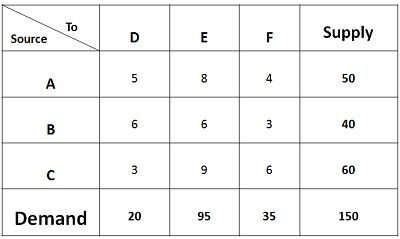
\includegraphics[width=7cm]{images/1.jpg}
	\caption{Csoportosítás indexelés nélkül}
	\label{fig:explain_2_1}
\end{figure}

A táblázatban három A, B és C forrás van megadva, amelyek termelési kapacitása 50 egység, 40 egység, illetve 60 egység termék. A három kiskereskedő D, E és F keresletét minden nap legalább 20 egység, 95 egység és 35 egység termékkel kell kielégíteni. A szállítási költségek szintén szerepelnek a mátrixban.

A szállítási feladat megoldásának előfeltétele, hogy a keresletnek meg kell egyeznie a kínálattal. Ha a kereslet nagyobb, mint a kínálat, akkor a táblázatba dummy-eredetet kell beilleszteni. A fiktív származási hely kínálata megegyezik a teljes kínálat és a teljes kereslet különbségével. A fiktív eredethez kapcsolódó költség nulla lesz.

Hasonlóképpen, ha a kínálat nagyobb, mint a kereslet, akkor létre kell hozni egy fiktív forrást, amelynek kereslete megegyezik a kínálat és a kereslet különbségével. A fiktív forráshoz kapcsolódó költség ismét nulla lesz.

Ha a kereslet és a kínálat megegyezik, a következő eljárást kell követni:

\begin{figure}[h!]
	\centering
	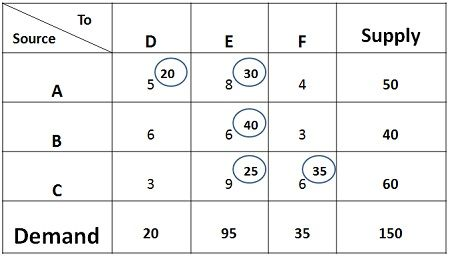
\includegraphics[width=7cm]{images/2.jpg}
	\caption{Csoportosítás indexelés nélkül}
	\label{fig:explain_2_1}
\end{figure}

Válassza ki a mátrix északnyugati vagy bal szélső sarkát, és a keresleti és kínálati korlátok között a lehető legtöbb egységet rendelje az AD cellához. Például 20 egységet rendelünk az első cellához, amely kielégíti a D célállomás keresletét, miközben a kínálat többletet mutat.
Most mozogjon vízszintesen, és rendeljen 30 egységet az AE cellához. Mivel 30 egység áll rendelkezésre az A forrással, a kínálat teljesen telítetté válik.
Most mozogjunk függőlegesen a mátrixban, és rendeljünk 40 egységet a BE cellához. A B forrás kínálata szintén teljesen telítetté válik.
Ismét lépjünk függőlegesen, és rendeljünk 25 egységet a CE cellához, az E célállomás kereslete teljesül.
Mozogjunk vízszintesen a mátrixban, és rendeljünk 35 egységet a CF cellához, mind a forrás, mind a célállomás kereslete és kínálata telítődik. Most már kiszámítható a teljes költség.

A teljes költség kiszámítható az egyes cellákhoz rendelt egységek és az érintett szállítási költség szorzataként. Ezért,

Teljes költség = 20*5+ 30*8+ 40*6+ 25*9+ 35*6 = 1015.


















